\underline{Solving Linear Inequalities}

A feature of linear inequalities is that the set of solutions will be an \emph{interval.} An interval is a set of all the points which satisfies a certain kind of inequality. There are nine different types of intervals.

\emph{The nine types of intervals}
\begin{gather*}
    \left[a,b\right] = ``\textrm{the set of all} \ x \ \textrm{that satisfy} \ a\le x \le b'' \\
    \left(a,b\right) = ``\textrm{the set of all} \ x \ \textrm{that satisfy} \ a< x < b'' \\
    \left(a,b\right] = ``\textrm{the set of all} \ x \ \textrm{that satisfy} \ a < x \le b'' \\
    \left[a,b\right) = ``\textrm{the set of all} \ x \ \textrm{that satisfy} \ a\le x < b'' \\
    \left[a,\infty\right) = ``\textrm{the set of all} \ x \ \textrm{that satisfy} \ a\le x'' \\
    \left(a,\infty\right) = ``\textrm{the set of all} \ x \ \textrm{that satisfy} \ a < x'' \\
    \left(-\infty,a\right] = ``\textrm{the set of all} \ x \ \textrm{that satisfy} \ x \le a'' \\
    \left(-\infty,a\right) =``\textrm{the set of all} \ x \ \textrm{that satisfy} \ x < a'' \\
    \left(-\infty,\infty\right) = ``\textrm{the set of all real numbers}''
\end{gather*}

The numbers \(a\) and \(b\) are called the \emph{endpoints} of the interval. In the notation for the interval, we use a \((\) or \()\) in association with \(<\). This amounts to the corresponding endpoint \emph{not} being included in the interval. We use \([\) or \(]\) in association with \(\le.\) This means that the corresponding endpoint will be in the interval. The symbols \(\infty, -\infty\) do not represent numbers and so it can never be the case that \(x=\infty.\) However, we may interpret \(x < \infty\) as ``\(x\) is finite.'' This applies to \emph{all} real numbers. Hence, \(a <x <\infty\) is the same as \(a<x.\) This is why we have infinity with the parentheses and \emph{never} a square bracket.

\begin{question} \label{LI1}
    Solve for \(x:\) \(3x-1>1\)

    \begin{solution}
        \begin{gather*}
            3x-1>1\\
            3x>2 \\
            x>\frac{2}{3}
        \end{gather*}
        The set of solutions is the set of all \(x\) greater than \(\frac{2}{3}.\)
        In interval notation, \(\left(\frac{2}{3},\infty\right)\)
    \end{solution}
\end{question}

An illustration of the set of all solutions to question \ref{LI1}.
\begin{image}
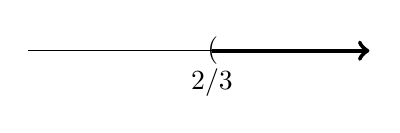
\begin{tikzpicture}
    \draw[-] (-5/3, 0) -- (8/3, 0);
    \draw[->,ultra thick] (2/3,0) -- (8/3,0);
    \node[below] at (2/3, -0.1) {$2/3$};
    \node at (2/3+0.01,0) {(};
    \end{tikzpicture}
\end{image}

\begin{question} \label{LI2}
    Solve for \(t:\) \(-\frac{1}{2}x+3\ge0\)

    \begin{solution}
        \begin{gather*}
            -\frac{1}{2}x+3\ge0\\
            -\frac{1}{2}x\ge-3 \\
            x\le 6
        \end{gather*}
        The set of solutions is the set of all \(x\) less than or equal to \(6.\)
        In interval notation, \(\left(-\infty,6\right]\)
    \end{solution}
\end{question}

An illustration of the set of all solutions to question \ref{LI2}.
\begin{image}
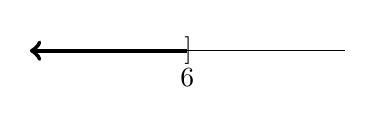
\begin{tikzpicture}
    \draw[-] (4, 0) -- (8, 0);
    \draw[<-,ultra thick] (4,0) -- (6,0);
    \node[below] at (6, -0.1) {$6$};
    \node at (6+0.01,0) {]};

    \end{tikzpicture}
\end{image}